% Chapter 1

\chapter{Beam position monitor} % Main chapter title

\label{Chapter6} % For referencing the chapter elsewhere, use \ref{Chapter1} 
One of the serious systematic error is beam position
We are developing Beam position monitor (BPM) for accurate measurement of beam position.
Previous study in LIGO have achieved 0.3~\% of uncertainty by using Telephoto camera system.
They place the telephoto camera at 8~m far from the ETM. On the other hand, That of KAGRA is 36 m where is 4.5 times larger. Therefore, one of the most difficult technologies of calibration is beam position measurement.

We will demonstrate the system of BMS as  the new technology. The BMS system is consists of 3 parts as shown in Fig.XXXX.

According to Eq.(\ref{eq:dx}), vector $\vec{a}$ and $\vec{b}$ corresponds to the rotation effect. $\vec{a}$ can be written as
\begin{equation}
\vec{a}=\vec{a_1} + \vec{a_2},
\end{equation}
where $\vec{a_1}$ and $\vec{a_2}$ are position vectors of two Pcal beams. We can measure the beam position of main interferometer, $\vec{b}$, as well.
We can obtain the rotation term as
\begin{equation}
\frac{I}{M}\vec{a} \cdot \vec{b}
\end{equation}
,where $I$ and $M$ are inertial moment and mass of test mass.

Furthermore, the misaligned beam positions make the elastic deformation on the mirror surface due to asymmetry. It is one of the serious systematic errors.
Detail of the elastic deformation is described in Sec.~\ref{Chapter4}.

\section{Instlation}
The installation phase of beam position monitor consists of two phases.
In first phase, we place the TCam system at the side of EXA and EYA chamber.
Detail of TCam is described in XXX. We connect the TCam and control PC (Raspberry pi) and operate it.
The purpose of TCam is not only calibration work but also other application.
We will monitor the pollution of water due to cryo-pumping effect. The taken picture will be analyzed automatically.
In second phase, we place the QPD and the pico motor. We will control the beam position using these components.
\section{Operation}
All the system is operated by MEDM system as shown in Fig.XXX.
For monitoring the beam position, we use two pictures, which are with and without illuminator. We use the is Open Source Computer Vision Librarly (OpenCV) in python for image analysis, which is a library for open source computer vision developed and released by Intel.
The operation strategy is listed as follows:
\begin{enumerate}
 \item Take a picture with illuminator. We set the integration time to 30 sec.
  \item Convert picture to gray scale.
  \item Set the reasonable threshold to find a boundary of beams and edge of ETM. 
   \item Mask the analysis region to separate the beam shape and ETM edge.
 \item Estimate the origin of mirror coordinate by fitting of edge shape of the mirror.
 \item Turn off the illuminator and take picture with 30 sec integration time.
  \item Estimate the Pcal beam position and main interferometer position with no illumination picture.
   \item Make a picture overplayed the coordinate of Pcal and origin as shown in Fig.~\ref{fig:Beam_mon}.
   \end{enumerate}
   \begin{figure}
\begin{center}
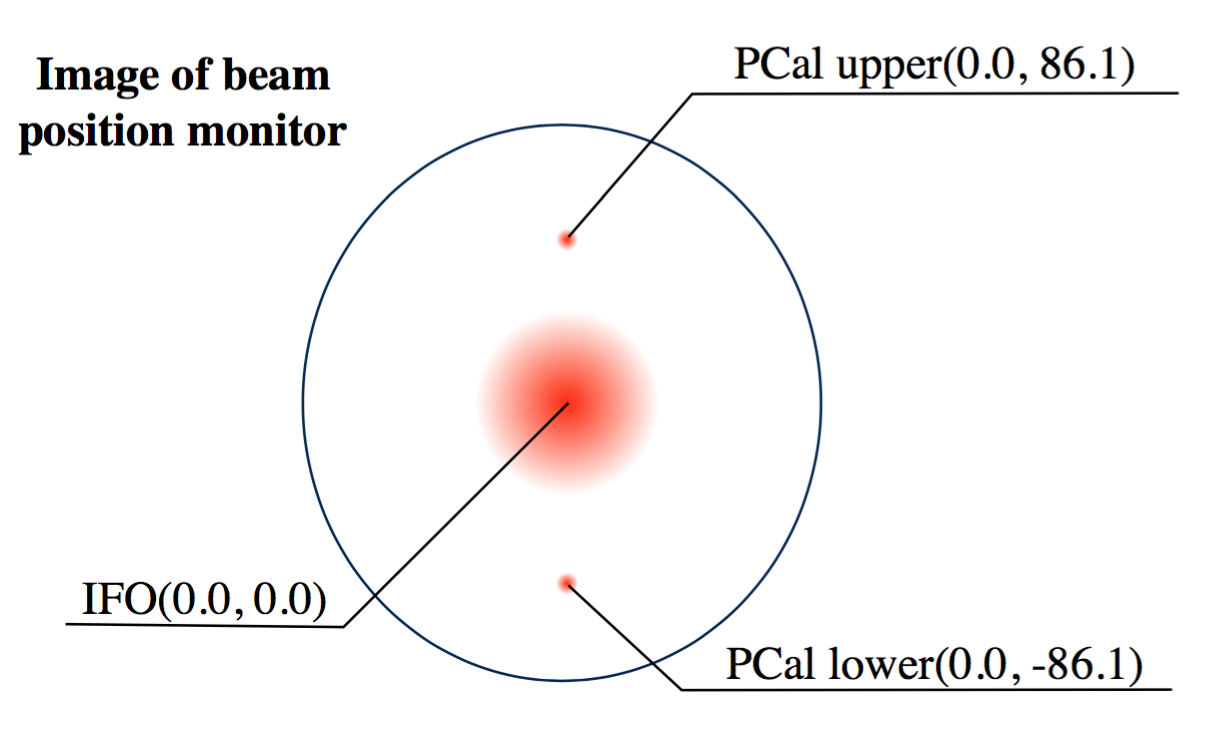
\includegraphics[width=14cm]{Figures/Beam_mon.eps}
\caption{Image of beam position monitor. We will over-plot the estimated beam position on the picture.} 
\label{fig:Beam_mon} 
\end{center}
\end{figure}


\section{Demonstration test}
We tried the demonstration test using Telephoto camera with 150mm diameter mirror and dummy target.
Figure XXX shows the test setup. We mount the target structure on the camera tripod. The size of target is $24 \times 24$~mm as shown in Fig XXX. The taken picture is shown in Fig XXX.
We are trimming the target region as shown in Fig. XXX. The trimmed data is converted to gray scale. We set the threshold point at 228.
Fig.~\ref{fig:Fiiting_terget} shows the datas over the threshold.
We masked the data points as shown in Fig.~\ref{fig:Analysis_cam}.
Finally, we have done a fitting and estimate the center point of the circle as shown in Table. XXXX.
Then, we assumed the following equation:
\begin{equation}
y=\sqrt{r-(x-x_0)}+y_0.
\end{equation} 
The measured and expected parameters are consistent within 1 sigma error.
Therefore, It imply that we can estimate the center point with 0.1 mm resolution.
In the KAGRA, we use smaller telescope of 127mm diameter.
We estimate the resolution when we use 127 mm telescope.
The estimated resolution is $\times 150/127=$. It meet our requirement.

   \begin{figure}
\begin{center}
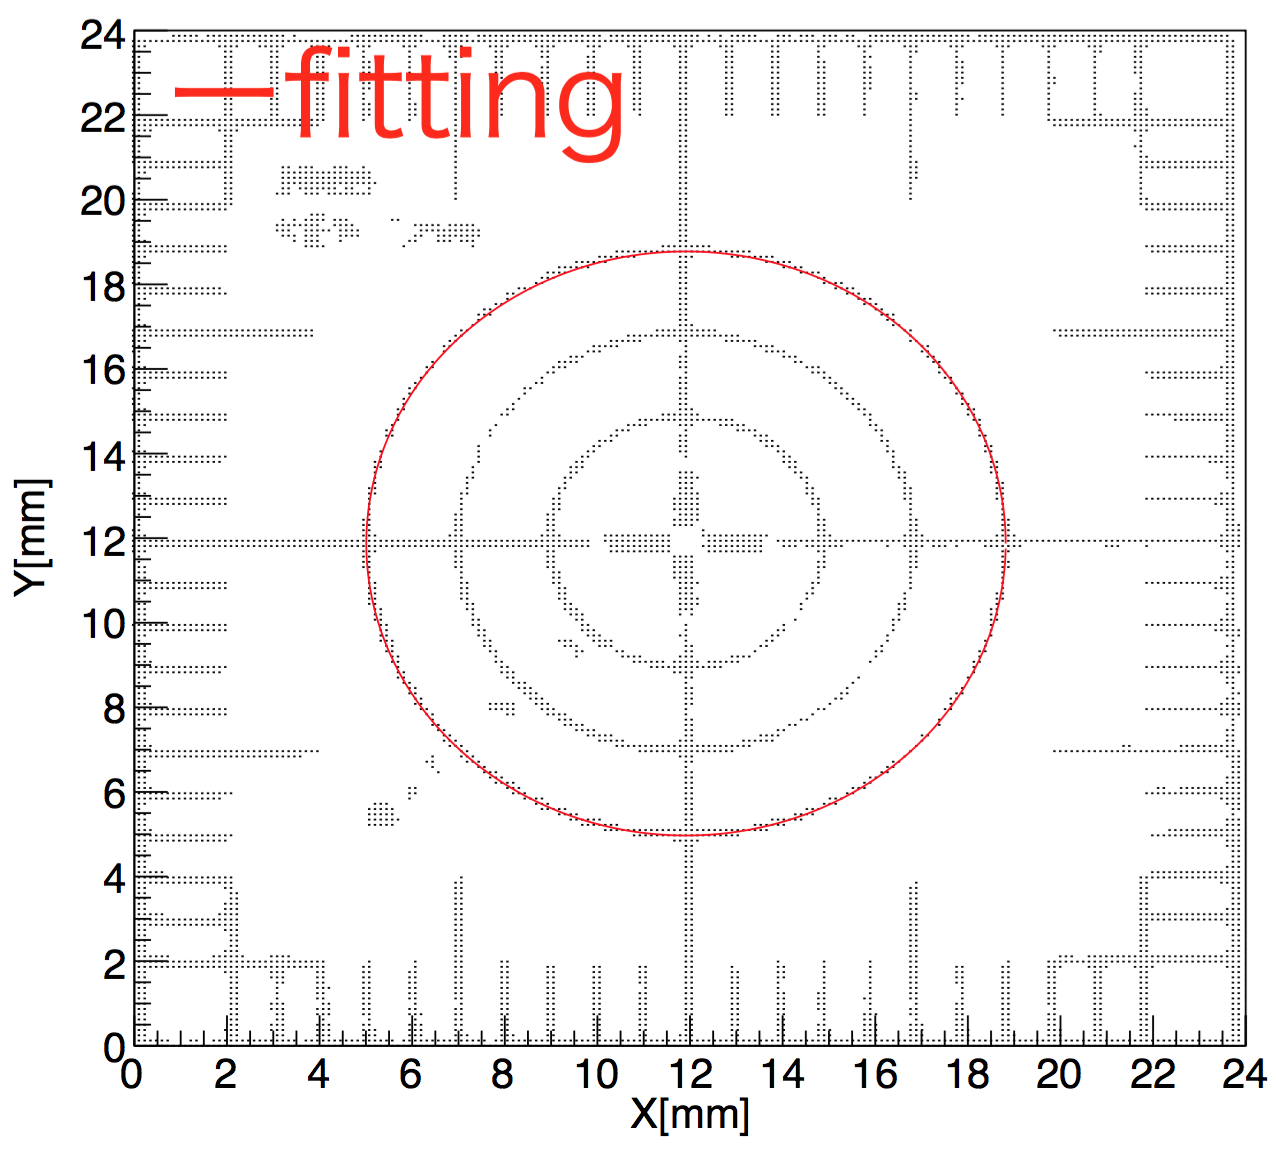
\includegraphics[width=14cm]{Figures/Fitting_target.eps}
\caption{.} 
\label{fig:Fitting_target} 
\end{center}
\end{figure}
   


   \begin{figure}
\begin{center}
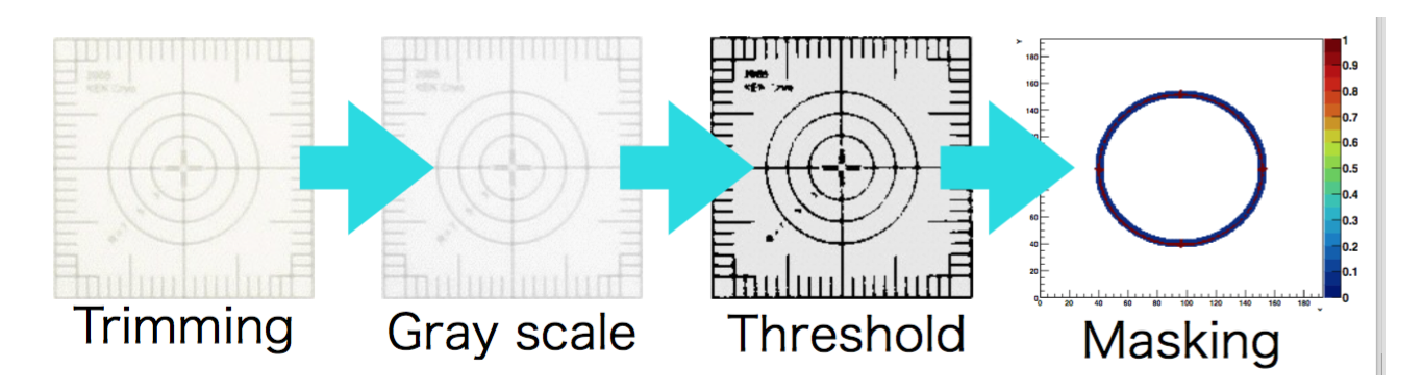
\includegraphics[width=14cm]{Figures/Analysis_cam.eps}
\caption{.} 
\label{fig:Analysis_cam} 
\end{center}
\end{figure}

\section{Summary}

 